\documentclass{standalone}
\usepackage{tikz}
\usepackage{ctex,siunitx}
\usepackage{tkz-euclide}
\usepackage{amsmath}
\usetikzlibrary{patterns, calc}
\usetikzlibrary {decorations.pathmorphing, decorations.pathreplacing, decorations.shapes,}
\begin{document}
	\small
	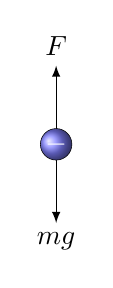
\begin{tikzpicture}[>=latex,scale=1]
		\draw [->] (0,0) -- (0,1);
		\draw [->] (0,0) -- (0,-1);
		\draw[very thin,ball color=blue!50,shading angle=20] (0,0) circle (0.2) node[text=white,scale=1.0] { $-$};
		\node at (0,1) [above] {$F$};
		\node at (0,-1) [below] {$mg$};
	\end{tikzpicture}
\end{document}